\documentclass[a4paper,11pt]{article}
\usepackage[utf8]{inputenc}
\usepackage[T1]{fontenc}
\usepackage[french]{babel}
\usepackage[right=2.5cm, left=2.5cm, bottom=4cm, top=3cm]{geometry}
\usepackage{textcomp}
\usepackage{graphicx}
\usepackage{mathtools,amssymb,amsthm}
\usepackage{lmodern}
\usepackage{multirow}
\usepackage{array}
\usepackage{longtable}
\usepackage{wrapfig}
\usepackage{amsmath}

\title{\vspace{13em}{\huge Manuel d'utilisation}}
\author{Edouard Fouassier - Maxime Gonthier - Benjamin Guillot\\
		Laureline Martin - Rémi Navarro - Lydia Rodrigez de la Nava
		\vspace{2em}\\
		Algorithme Génétique
		\vspace{2em}}

\begin{document}
\pagenumbering{gobble}\clearpage\pagenumbering{arabic}
	\maketitle\vspace{13em}
\newpage
\tableofcontents
\newpage\clearpage

\section{Installation}
Pour installer les prérequis, une commande vous est fournie permettant une installation simple.\\
Pour cela il suffit de vous placer, via le terminal, dans le dossier du programme \\
et d'effectuer la commande suivante : \textit{make install}\\
\begin{tabbing}
Cela exe\=cute les commandes :\\
		\>\textit{sudo apt-get update}\\
		\>\textit{sudo apt-get install qtbase5-dev}\\
		\>\textit{sudo apt-get install texlive-full}\\
		\>\textit{sudo apt-get install texlive-latex-extra}\\
		\>\textit{sudo apt-get install texlive-lang-french}\\
		\>\textit{sudo apt-get install gnuplot}\\
\end{tabbing}
Permettant respectivement de mettre à jour, installer QT5, le necessaire pour les fichiers de sortie $.tex$ et $.fig$.\\


\section{Présentation de l'interface}
Pour lancer le programme il suffit d'effectuer la commande : \textit{make run}.\\
Lors de l'ouverture du programme la fenêtre d'interface suivante apparaît :\\
\centerline{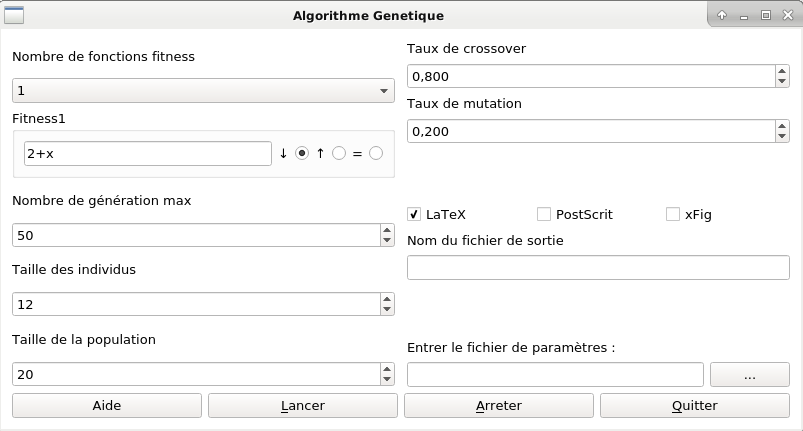
\includegraphics[scale = 0.5]{screen1.png}}


\newpage
\vspace{-1.5cm}
\begin{wrapfigure}[29]{r}{0.5\textwidth}
  \begin{center}
  \vspace{-2cm}
    \frame{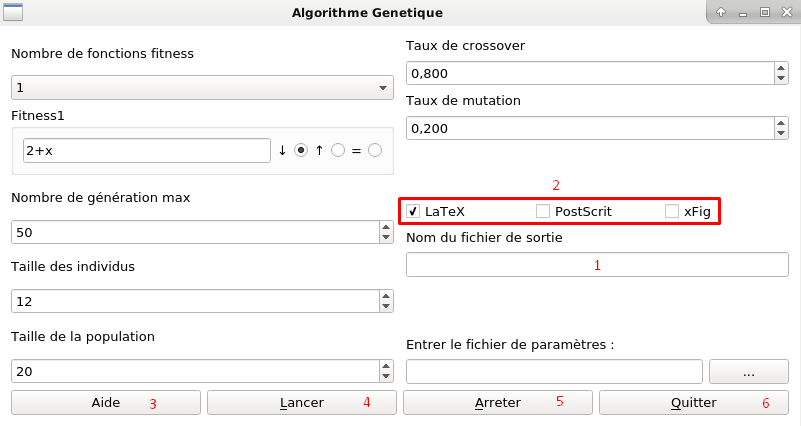
\includegraphics[scale=0.3]{screen2.png}}
  \end{center}
    \vspace{-1cm}
    \begin{center}
    \frame{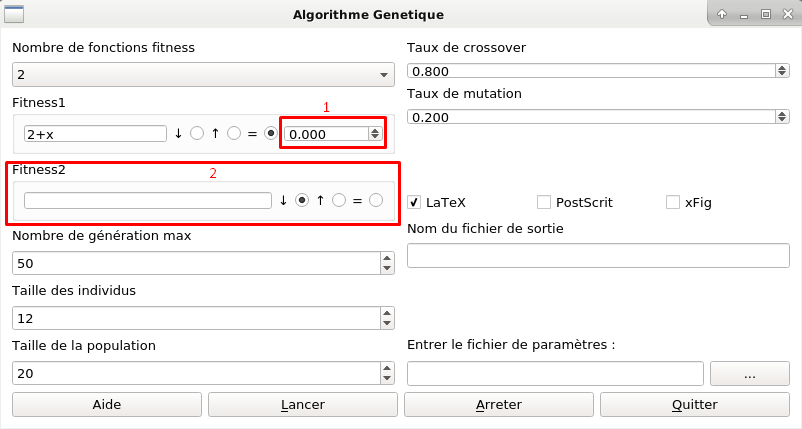
\includegraphics[scale=0.3]{screen3.png}}
  \end{center}
      \vspace{-1cm}
  \begin{center}
    \frame{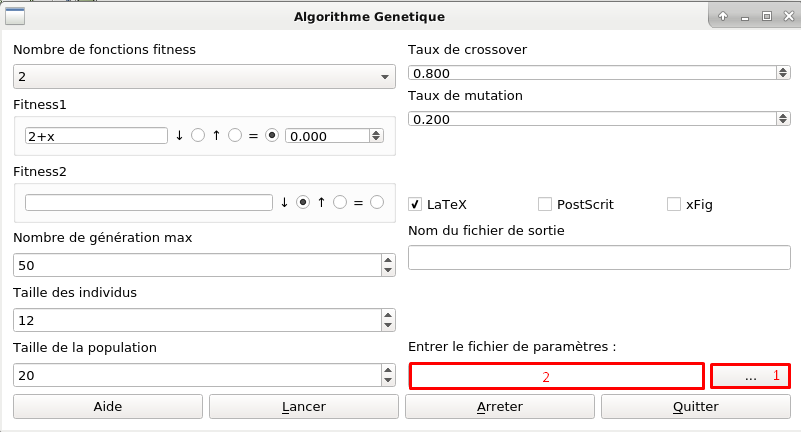
\includegraphics[scale=0.3]{screen4.png}}
  \end{center}
      \vspace{-1cm}
  \begin{center}
    \frame{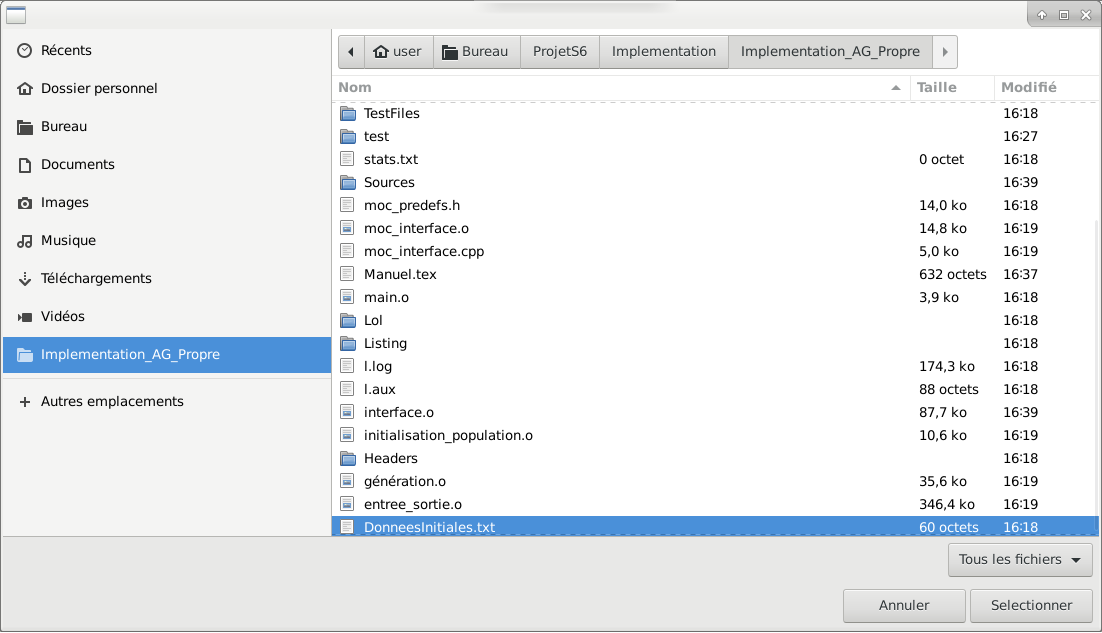
\includegraphics[scale=0.22]{screen5.png}}
  \end{center}
      \vspace{-1cm}
  \begin{center}
    \frame{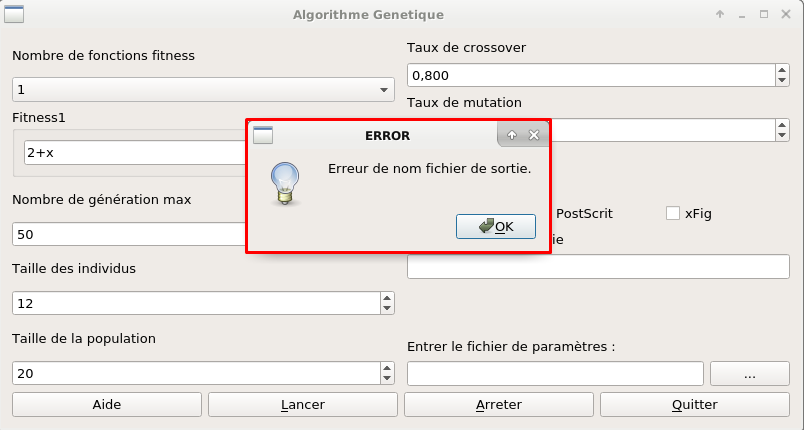
\includegraphics[scale=0.3]{screen6.png}}
  \end{center}
\end{wrapfigure}
Le programme est déjà presque pret à être lancé avec des paramètres par défaut. Il vous suffit de remplir le champ \textit{(1)Nom du fichier de sortie} et sélectionner les options de sortie (2). Ces données sont nécessaires à chaque lancement et le nom doit être unique. \\
\vspace{0.6cm}

Vous pouvez personnaliser l'algorithme grâce au différents champs mis à disposition. Si pour la fonction fitness, l'option de valeur approchée (=) est sélectionnée, un champ de saisie de cette valeur apparaitra(1).
Si vous choisissez d'avoir deux fonction fitness, une partie dédié ea celle-ci apparaitra aussi(2).\\

\vspace{1.2cm}

Vous pouvez aussi charger un fichier en cliquant sur le bouton (1) à droite du champ \textit{Entrer le fichier de paramètre}(2). Cela ouvrira une fenêtre permettant de trouver votre fichier de paramètre.\\

\vspace{2.5cm}

Dans cette fenètre vous pouvez parcourir tout vos dossiers afin de sélectionner votre fichier.\\

\vspace{3.5cm}

Si vous avez fait une erreur de paramètre, que ce soit par l'interface ou via un fichier, elle sera détectée et indiquée.\\


\section{Fichier de données}
Pour executer le programme deux méthodes sont disponibles : soit en entrant les paramètres via les champs de l'interface, soit via un fichier de données fourni par l'utilisateur.\\
Dans cette seconde option, le fichier devra imperativement respecter le format suivant : \\
\begin{itemize}
 \item Taille d'un individu en nombre de bits (de 1 à 32), bit de signe non inclu.
 \item Taux de mutation (0 à 1)
 \item Taux de crossover (0 à 1)
 \item Taille de la population (2 à 100)
 \item Nombre maximum de génération (1 à 1000)
 \item Nombre de critères (1 ou 2)
 \item Première fonction fitness (voir partie 4 du manuel d'utilisation page xx)
 \item Critère de la première fonction fitness (1=maximisation 2=minimisation 3=utilisation d'une valeur approchée)
 \item Valeur approchée de la première fonction fitness (-1000 à 1000, inutile si critère différent de 3)
 \item Deuxième fonction fitness (voir partie 4 du manuel d'utilisation page xx, inutile si il n'y a qu'un critère)
 \item Critère de la deuxième fonction fitness (1=maximisation 2=minimisation 3=utilisation d'une valeur approchée, inutile si il n'y a qu'un critère)
 \item Valeur approchée de la deuxième fonction fitness (-1000 à 1000, inutile si critère différent de 3, inutile si il n'y a qu'un critère)
 \item Les formats de fichier de sortie du programme sous forme de 3 chiffres, 1 ou 0, si on veux ou non une sortie de ce format (latex postscript xfig)
 \end{itemize}
 Les valeurs inutiles ne génèrent pas d'erreur.\\
 Des fichiers d'exemples sont fournis.\\

\newpage
\section{Fonction fitness}
	\underline{Symboles :}\\
\begin{tabbing}
A écrire	\hspace{0.5cm} \=	\hspace{1cm}  \=Ce à quoi ça correspond\\
2 + 1		\>-> \>2 plus 1\\
2 - 1		\>-> \>2 moins 1\\
2 * 1		\>-> \>2 fois 1\\
2 / 1		\>-> \>2 divisé par 1 (mettre des parenthèses si il y a un calcule sous le division)\\
-2			\>-> \>moins 2\\
2, 1		\>-> \>1\\
2\^{}1			\>-> \>2 puissance 1\\
2\%1		\>-> \>2 modulo 1\\
\end{tabbing}

	\underline{Fonctions :}\\
\begin{tabbing}
A écrire	\hspace{0.5cm} \=	\hspace{1cm}  \=Ce à quoi ça correspond\\
abs			\>->	\>Valeur absolue\\
acos		\>->	\>arc cosinus\\
asin		\>->	\>arc sinus\\
atan		\>->	\>arc tangente\\
atan2		\>->	\>arc tangente avec 2 arguments\\
ceil		\>->	\>valeur entière supérieure\\
cos			\>->	\>cosinus\\
cosh		\>->	\>cosinus hyperbolique\\
e			\>->	\>exponentielle = 2.718281...\\
exp			\>->	\>exponentielle avec un exposant après\\
floor		\>->	\>valeur entière inférieure\\
ln			\>->  \>logarithme neperien\\
log			\>->  \>logarithme\\
log10		\>->	\>logarithme en base 10\\
pi			\>->	\>Pi = 3.141591...\\
pow			\>->	\>puissance, s'écrit pow(10, 2) pour 10\^{}2\\
sin			\>->	\>sinus\\
sinh		\>->	\>sinus hyperbolique\\
sqrt		\>->	\>racine carré\\
tan			\>->	\>tangente\\
tanh		\>->	\>tangente hyperbolique\\
\end{tabbing}
Pour une plus simple utilisation nous conseillons de bien parenthèser les équations.\\

\section{Exploitation des résultats}
Lors de sont éxécution, le programme crée un dossier comportant plusieurs fichiers nommés à partir du nom donné par l'utilisateur.\\
\begin{tabbing}
Les fichiers suivant seront générés \=à chaque\= lancement et sont utilisés par le programme : \\
nom\_Populations.txt : \> regroupant les scores de chaque individu à chaque génération.\\
nom\_Parametres.txt : \>	regroupant les paramètres donnés par l'utilisateurs.\\
nom\_Stats : \> regroupant les statistiques des scores de chaque génération. \\
\>\>(moyenne maximum minimum)\\\\
\end{tabbing}
De plus, des fichiers seront générés à la demande de l'utilisateur, en .tex, .fig ou .ps.\\
Si l'utilisateur désire générer un fichier PDF  à partir du .tex ou .ps, nous recommandons l'utilisation de la commande \textit{pdflatex nom.tex} et \textit{ps2pdf nom.ps}.\\
Les PDF présenteront les paramètres entrés par l'utilisateur, un ou deux graphiques représentants l'évolution des scores minimum, maximum et la moyenne réduite.\\
Ainsi qu'un tableau des 10 meilleurs individus (solutions) et un tableau complet de l'évolution des scores à chaques générations.\\
Pour l'exploitation du .fig nous recommandons le logiciel Dia.\\
Il permet la visualisation des graphiques représentants l'évolution des scores minimum, maximum et la moyenne réduite.\\

	
\end{document}

